%% Los cap'itulos inician con \chapter{T'itulo}, estos aparecen numerados y
%% se incluyen en el 'indice general.
%%
%% Recuerda que aqu'i ya puedes escribir acentos como: 'a, 'e, 'i, etc.
%% La letra n con tilde es: 'n.

\chapter{Introducción}

La teledetección constituye una herramienta de gran utilidad para el desarrollo de sistemas de prevención, seguimiento y evaluación de superficie terrestre. Se define como  la  técnica  que  permite  adquirir  imágenes  de  la  superficie terrestre desde sensores instalados en plataformas espaciales o aereotransportadas. Este proceso se basa en la detección y medición de radiación electromagnética emitida ya sea de manera natural o a partir de una fuente artificial emisora. La energía es captada por sensores y permite identificar objetivos por sus propiedades físicas y sustancias que lo componen. Estos sensores emiten radiación electromagnética comprendida en varias zonas del espectro electromagnético. La parte del espectro electromagnético usada en teledetección se extiende aproximadamente desde $10^{-1} \mu m$ hasta $10^{9} \mu m$, donde $\mu m$ se llama al  micrómetro que es la millonésima parte del metro.

Esta técnica de teledetección comprende dos procesos. Uno de estos procesos es la adquisición de información de la superficie terrestre captando la radiación electromagnética emitida o reflejada por ésta. El otro es el almacenamiento de la información obtenida para su posterior procesamiento en virtud de interpretarla y utilizarla. 

El sensor remoto recibe la radiación que proviene de los objetos situados sobre la superficie terrestre. En función de la forma en la que se refleje esta radiación podremos clasificar los distintos tipos de terrenos.

%\begin{figure}[hbt]
%	\centering    
%	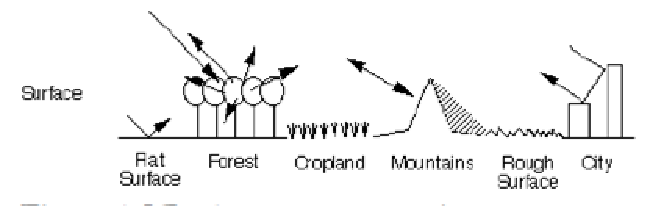
\includegraphics[scale=0.7]{../../Figures/Tesis/Capitulo4/Backscatter.pdf}
%	\caption{\label{Backscatter}Radiación reflejada por distintos objetos en la superficie terrestre.}
%\end{figure} 

Los sistemas de teledetección se pueden dividir principalmente en dos grupos: los teledetectores activos y los pasivos. Los sensores activos tienen su propia fuente de energía para iluminar los objetos que observan. Ellos emiten radiación en la dirección del objetivo a ser investigado, detecta y mide la radiación que es reflejada o retrodispersada desde el objetivo. Los sensores pasivos, por otra parte, detectan la radiación electromagnética emitida o reflejada de fuentes naturales, no necesitan una fuente de energía externa. La luz del sol reflejada es la fuente más común de la radiación medida por los sensores pasivos. Un ejemplo de sensor pasivo es el espectrómetro óptico o espectroscopio, que es un instrumento que sirve para medir las propiedades de la luz en una determinada porción del espectro electromagnético. El Radar es un ejemplo de sensor activo.

%Entre las ventajas que ofrece la Teledetección, destaca su alta periodicidad temporal, por lo que se facilita el seguimiento de aquellas variables ambientales sometidas a una intensa dinámica. Además, gracias a la teledetección ambiental se brinda la posibilidad de obtener información de grandes superficies de territorio en poco tiempo, de tal manera que extensas regiones pueden ser muestreadas en su totalidad en pocos días.

Los sistemas de Radar (radio detection and ranging: detección y medición de distancias por radio) son instrumentos que, a través de ondas electromagnéticas, detectan un objeto e indican su distancia y posición. Estos instrumentos miden la respuesta del terreno a la radiación electromagnética emitida en forma de pulsos, el valor de esta respuesta es almacenada para su posterior procesamiento y se utiliza para formar una imagen de la zona de interés. Un Radar de Apertura Sintética (synthetic aperture radar: SAR) es un tipo de sistema que consiste en procesar, mediante algoritmos, la información capturada por la antena del radar. Mediante este proceso se consigue el mismo rendimiento que se obtendría si se utilizara una antena mucho más grande que la que tiene en realidad, por eso se llaman de apertura sintética. 

Los dispositivos de captura de imágenes que emplean iluminación coherente, como sucede en las imágenes de ultrasonido B, laser y de radar de apertura sintética – SAR (Synthetic Aperture Radar ) entre otros, introducen un ruido que es propio del sistema de captura de la imagen. Este ruido, llamado speckle, no es gaussiano ni aditivo y, por lo tanto, diferente al ruido que se observa en imágenes ópticas. Existen diferentes técnicas para disminuir la presencia de este ruido, pero como contrapartida la imagen pierde resolución.

La utilización de modelos estadísticos ha sido una herramienta fundamental para analizar e interpretar datos con ruido speckle. Se han presentado varias distribuciones para modelar este tipo de imágenes. Las distribuciones Lognormal y Weibull fueron introducidas para caracterizar datos de alta resolución~\cite{oliverquegan98}, las distribuciones \textit{K} y Weibull también fueron estudiadas en~\cite{Oliver1993}, en~\cite{Tison2004} los autores presentaron la distribución de Fisher para modelar varios tipos de áreas. Li et al.~\cite{Li2011} propusieron una distribución Gamma generalizada para modelar imágenes SAR que tiene las distribuciones Weibull, \textit{K} y Fisher, entre otras, como casos particulares. Cabe señalar que la distribución $\mathcal{G}^0$ está relacionada con la distribución de Fisher~\cite{MejailJacoboFreryBustos:IJRS}.

El modelo propuesto para datos provenientes de un sistema de iluminación por radiación coherente, como son los datos SAR, es un modelo multiplicativo que considera que el valor observado en cada celda de la imagen es una variable aleatoria $Z$ que resulta del producto de dos variables aleatorias independientes: una correspondiente a la retrodispersión $X$ (que es lo que observaríamos sin la presencia del ruido speckle) y la otra correspondiente al ruido speckle $Y$ (que es inherente a todo sistema de captura de imágenes con iluminación coherente)~\cite{oliverquegan98}. 

En los últimos años, se ha utilizado exitosamente el modelo $\mathcal{G}^0$: $\mathcal{G}_A^0$ para datos de amplitud y $\mathcal G_I^0$ para datos de intensidad, porque tiene la capacidad de discriminar áreas muy texturadas o extremadamente texturadas mejor que otros modelos. Este modelo fue propuesto por Frery et al. \cite{Frery97} y está caracterizado por tres parámetros; el parámetro $\alpha$ que explica la textura, el parámetro $\gamma $ que informa sobre el brillo de la imagen y el número de looks $L$ que está relacionado con la relación señal-ruido.
Debido a esta interpretabilidad, es crucial obtener estimaciones de calidad de dichos parámetros, en particular para $\alpha$.

Varios autores han estudiado el problema de la estimación de parámetros para la familia $\mathcal G^0$. Freitas et al.~\cite{Freitas2005} usaron el primer y segundo momento para estimar los parámetros de textura y escala en el caso de datos de intensidad.
Vasconcellos et al.~\cite{VasconcellosFrerySilva:CompStat} cuantifican el error en la estimación del parámetro de textura para la distribución $\mathcal G_A^0$ y proponen una técnica analítica para mejorar la estimación a través de una corrección de segundo orden en el sesgo de la estimación del parámetro de textura. Li et al~\cite{Li2011} obtuvieron una expresión para los estimadores de la distribución Gamma generalizada basada en cumulants de segundo tipo y una aproximación de segundo orden de la función Polygamma. Cribari-Neto et al.~\cite{CribariFrerySilva:CSDA} implementaron técnicas de remuestreo para mejorar la estimación de parámetros para el modelo $\mathcal G_I^0$.

Nicolas y Anfinsen~\cite{nicolas2002} propusieron el método basado en Logmomentos y Logcumulantes para estimar los parámetros de una distribución. Estos métodos dependen de la relación entre los momentos de la distribución y su transformada de Mellin. La misma idea fue aplicada por Khan y Guida~\cite{khan2014} para estimar los parámetros del modelo $\mathcal{G}$ multivariado en el caso de datos SAR polarimétricos y también fue utilizada por Tison et al.~\cite{Tison2004} para la estimación del modelo $\mathcal{G}$ para datos de amplitud.

Unas de las propiedades deseables para un estimador es su robustez, esto es, su capacidad para dar buenas estimaciones aún en presencia de datos atípicos. Bustos et al.~\cite{BustosFreryLucini:Mestimators:2001} y Allende et al.~\cite{AllendeFreryetal:JSCS:05} propusieron M y AM estimadores para mejorar el comportamiento del estimador de Máxima Verosimilitud bajo contaminación. Ellos mostraron que su propuesta, si bien supera la performance del estimador de Máxima Verosimilitud, presenta problemas numéricos especialmente para el caso de muestras de pequeño tamaño.

Por otro lado, la teoría de la información ha sido aplicada a los métodos de estadística y probabilidades con éxito~\cite{Liese2006}. 
Shannon~\cite{Shannon1948} definió la información $I(X,Y)$ entre las variables aleatorias $X$ e $Y$ como una divergencia calculada entre sus densidades de probabilidad. 
Estas divergencias fueron ampliamente estudiadas por Kullback y Leibler~\cite{KullbackLeibler1951} y por Rényi~\cite{renyi1961} entre otros y es una medida de la distancia entre dos funciones de densidad. 
%El concepto de divergencias como distancias estocásticas se describe detalladamente en~\cite{Liese2006}, así como también sus propiedades.  
% Mejorar las referencia en eventos con artigos en periódicos
Este tipo de divergencias poseen múltiples aplicaciones en procesamiento de señales e imágenes~\cite{Aviyente2007}, análisis de imágenes médicas~\cite{5599869},
clasificación de texturas~\cite{1246862}, restauración de imágenes~\cite{1224731} e incluso en detección automática de regiones con diferente grado de rugosidad en imágenes SAR~\cite{6377288,ClassificationPolSARSegmentsMinimizationWishartDistances}.


Los estimadores de mínima distancia (MDE) son una  alternativa con buenas propiedades para el problema de la estimación de parámetros.
Surgen de la idea de encontrar un estimador que sea el valor que minimiza la medida de la distancia entre las funciones de distribución empírica y teórica.
Wolfowitz~\cite{wolfowitz1953, wolfowitz1957} estudió esta clase de estimadores y demostró que, bajo condiciones generales, estos estimadores son fuertemente consistentes. 
Boos~\cite{Boos1981} estudió la distancia ponderada de Cramer-von Mises entre la función de distribución empírica y el modelo verdadero.
El autor mostró que estos estimadores son consistentes y asintóticamente eficientes bajo cierta función de peso.
Hettmansperger et al.~\cite{HettmanSperger1994} estudiaron estimadores de mínima distancia no pesados aplicados a un modelo de posición-escala a partir de la distancia de Cramer-von Mises. El autor demostró que estos estimadores son asintóticamente normales y tienen buenas propiedades de eficiencia y robustez.
Beran~\cite{beran1977} propone un MDE estimador utilizando la distancia de Hellinger entre un modelo teórico y un estimador de densidad no paramétrico utilizando núcleos simétricos y mostró que este estimador es asintóticamente eficiente bajo ciertas familias paramétricas de densidades.
Parr y Schucany~\cite{parr1982} demostraron que, considerando ciertas condiciones, el estimador MDE entre la función de distribución empírica y la función de distribución teórica es fuertemente consistente.

Cao et al.~\cite{cao1995minimum} propuso minimizar una distancia entre la función de densidad teórica y un estimador de la función de densidad subyacente utilizando el estimador de núcleo simétrico clásico para obtener estimadores de distancia mínima. Demostraron, siguiendo~\cite{parr1982}, la consistencia fuerte de estos estimadores bajo ciertas consideraciones, y también estudiaron su normalidad asintótica para el caso de la métrica $ L^2 $.

%Gambini et al.~\cite{gambini2015} propusieron un estimador del parámetro de textura de la distribución $\mathcal{G}_I^0$ combinando MDE con distancias estocásticas. 
%combining MDEs with stochastic distances. Ellos prponen minimizar la distancia triangular entre la función de densidad teórica y una estimación no paramétrica de la función de densidad subyacente utilizando núcleos asimétricos, en este caso, utilizaron el kernel gaussiano inverso. Los autores compararon el desempeño del estimador propueston con el obtenido por logcumulación y Máxima Verosimilitud, y obtuvieron buenos resultados
%en términos de error cuadrático medio, sesgo, consistencia y robustez. 

Dentro de los estimadores no paramétricos de la función de densidad subyacente se encuentran los estimadores de kernel clásico, con kernel simétrico~\cite{Silverman1986} que son populares en la estimación de la función de densidad. Sin embargo, si la función de densidad a estimar tiene soporte acotado, estos estimadores pueden dar estimaciones sesgadas en los bordes del soporte porque asignan probabilidad positiva fuera del soporte de la función. Una alternativa para mejorar esto es utilizar kernels asimétricos, Chen~\cite{chen1999, chensx2000} presenta núcleos Beta y Gamma, Scaillet~\cite {Scaillet2004} introduce núcleos Inverso Gaussianos (IG) y Recíproco Inverso Gaussiano (RIG), Bouezmarni et al.~\cite {bouezmarni2005} demuestran propiedades teóricas de los núcleos Gamma, IG y RIG. En~\cite{Jin2003} los autores proponen los núcleos Birnbaum-Saunders (BS) y Lognormal (LN). Es interesante señalar que  estos estimadores varían su forma de acuerdo con la observación, una característica que permite obtener diferentes grados de suavizamiento sin incurrir en los problemas antes mencionados~\cite{Scaillet2004}. 

En esta tesis se propone un nuevo  estimador de los parámetros de la distribución $\mathcal{G}_I^0$ definido como el punto del espacio paramétrico que minimiza la distancia estocástica que existe entre la función de densidad teórica $\mathcal{G}_I^0$ y una estimación no paramétrica de la función de densidad subyacente utilizando núcleos asimétricos. Se muestra que la distancia triangular es una buena elección para tratar este problema y se prueba la consistencia y la convergencia en casi todo punto de este estimador. Asimismo, a través de simulaciones Monte Carlo, se analiza:

\begin{itemize}
	\item El desempeño de este estimador para pequeñas muestras comparándolo, en términos de sesgo y error cuadrático medio y tasa de convergencia, con los estimadores presentes en la literatura.
	\item La robustez del estimador propuesto bajo diferentes esquemas de contaminación.
\end{itemize}  

Esta tesis está organizada de la siguiente manera:
\begin{itemize}
	\item En el capítulo~\ref{Radar} presentamos conceptos de teledetección y los radares de apertura sintética dando una breve reseña de principales sensores SAR. Presentamos también la generación de imágenes SAR y  la formación del ruido speckle.
	\item En el capítulo~\ref{modeloG0} se introduce el modelo multiplicativo base de la metodología adoptada para explicar el comportamiento de las imágenes SAR. Presentamos las distribuciones de cada una de las variables que forman parte del modelo multiplicativo y, finalmente, presentamos la familia de distribuciones $\mathcal{G}_I$ objeto de estudio en esta tesis.
	\item En el capítulo~\ref{metodologia}  se describen dos metodologías de estimación de la función de densidad, paramétrica y no paramétrica. Damos una descripción de cada una de estas metodologías y presentamos el principal aporte de esta tesis, que es la propuesta de un nuevo método de estimación para los parámetros del modelo $\mathcal G_I^0$.
	\item En el capítulo~\ref{ResultadosEmpiricos} se presenta el estudio realizado, a través de simulaciones Monte Carlo, del estimador propuesto. Se muestran los resultados obtenidos de estas simulaciones  con datos contaminados y sin contaminar, y la aplicación de estos métodos en imágenes reales.
	\item En el capítulo~\ref{ResultadosTeoricos} se presenta resultados de convergencia del estimador propuesto.
	\item En el capítlo~\ref{Conclusiones} se presentan las conclusiones finales de este trabajo.
	
\end{itemize}

